\documentclass[11pt]{article}
\usepackage[margin=1in]{geometry}
\usepackage{amsmath,amssymb,amsfonts,mathtools,bm}
\usepackage{booktabs}
\usepackage{tikz}
\usetikzlibrary{arrows.meta,positioning,shapes.geometric}
\usepackage{hyperref}

\title{TreeNB-VAE: Rigorous Theoretical Formulation}
\date{}

\begin{document}
\maketitle

\section{Setup}
Let $\mathcal{T}=(V,E)$ be a rooted taxonomy tree with $|V|=N$ nodes, $|E|=N-1$ directed parent$\to$child edges, and $L$ leaves.
For sample $i\in\{1,\dots,B\}$, observed leaf counts are
\[
\bm{x}^{(i)}=(x_1^{(i)},\dots,x_L^{(i)})\in\mathbb{N}_0^L,
\quad
s^{(i)}=\sum_{\ell=1}^L x_\ell^{(i)}.
\]
Encoder inputs are log-transformed counts
\[
\tilde{\bm{x}}^{(i)}=\log\big(\bm{x}^{(i)}+\varepsilon\big),\qquad \varepsilon>0.
\]

\section{Latent-variable model}
The model defines
\[
\bm{z}^{(i)}\sim\mathcal{N}(\bm{0},I_d),
\qquad
\bm{p}^{(i)}=f_{\text{tree}}(\bm{z}^{(i)})\in\Delta^{L-1},
\qquad
\mu_\ell^{(i)}=s^{(i)}p_\ell^{(i)}.
\]
Each leaf count is Negative Binomial:
\[
x_\ell^{(i)}\mid\bm{z}^{(i)}\sim\operatorname{NB}(\mu_\ell^{(i)},\theta_\ell),
\quad \ell=1,\dots,L.
\]
Per-feature inverse-dispersion is shared across samples:
\[
\theta_\ell=\exp(\eta_\ell),\quad \eta_\ell\in\mathbb{R}.
\]
The NB log-likelihood for $x\in\mathbb{N}_0$ is
\begin{align*}
\log p(x\mid\mu,\theta)
&=\log\Gamma(x+\theta)-\log\Gamma(\theta)-\log\Gamma(x+1)\\
&\quad+\theta\log\frac{\theta}{\theta+\mu}+x\log\frac{\mu}{\theta+\mu}.
\end{align*}
It yields
\[
\mathbb{E}[x]=\mu,
\qquad
\operatorname{Var}(x)=\mu+\frac{\mu^2}{\theta}.
\]

\section{Inference model}
The encoder is diagonal Gaussian:
\[
(\bm{\mu}_z,\log\bm{\sigma}_z^2)=g_\phi(\tilde{\bm{x}}),
\qquad
q_\phi(\bm{z}\mid\bm{x})=\mathcal{N}(\bm{\mu}_z,\operatorname{diag}(\bm{\sigma}_z^2)).
\]
Sampling is reparameterized:
\[
\bm{z}=\bm{\mu}_z+\bm{\sigma}_z\odot\bm{\epsilon},
\qquad \bm{\epsilon}\sim\mathcal{N}(\bm{0},I_d).
\]
KL to the standard normal prior is
\[
\mathrm{KL}(q_\phi\|p)
=\frac12\sum_{j=1}^d\left(\mu_{z,j}^2+\sigma_{z,j}^2-1-\log\sigma_{z,j}^2\right).
\]

\section{Tree-softmax decoder}
The decoder outputs edge logits $\bm{a}\in\mathbb{R}^{|E|}$:
\[
\bm{a}=h_\psi(\bm{z}).
\]
For each internal node $u$, define children set $\mathcal{C}(u)$ and sibling-normalized probabilities
\[
\pi_{u\to v}=
\frac{\exp(a_{u\to v})}{\sum_{v'\in\mathcal{C}(u)}\exp(a_{u\to v'})},
\qquad v\in\mathcal{C}(u).
\]
For leaf $\ell$ with unique root-to-leaf path $\mathcal{P}(\ell)$,
\[
p_\ell=\prod_{e\in\mathcal{P}(\ell)}\pi_e,
\qquad
\sum_{\ell=1}^L p_\ell=1.
\]

\subsection*{Path-matrix acceleration}
Define binary matrix $P\in\{0,1\}^{|E|\times L}$:
\[
P_{e\ell}=1\iff e\in\mathcal{P}(\ell).
\]
With edge log-probabilities $\bm{r}=\log\bm{\pi}\in\mathbb{R}^{|E|}$,
\[
\log\bm{p}=\bm{r}^\top P\in\mathbb{R}^L.
\]
Thus all leaves are computed by one matrix multiplication.

\section{Exact hierarchical consistency}
Because each internal node uses a softmax over its children,
\[
\sum_{v\in\mathcal{C}(u)}\pi_{u\to v}=1.
\]
Hence the induced mass decomposition satisfies
\[
\mathrm{mass}(u)=\sum_{v\in\mathcal{C}(u)}\mathrm{mass}(v)
\]
exactly, for all internal nodes $u$. Therefore parent-child consistency is structural, not penalized.

\section{$\beta$-ELBO objective}
Per sample loss:
\[
\mathcal{J}^{(i)}
=-\sum_{\ell=1}^L\log p\big(x_\ell^{(i)}\mid\mu_\ell^{(i)},\theta_\ell\big)
+\beta_t\,\mathrm{KL}\Big(q_\phi(\bm{z}^{(i)}\mid\bm{x}^{(i)})\,\|\,\mathcal{N}(\bm{0},I)\Big).
\]
Batch objective is the sample mean of $\mathcal{J}^{(i)}$.
Warmup schedule:
\[
\beta_t=\min\!\left(\beta_{\max},\,\beta_{\max}\frac{t}{T_{\text{warmup}}}\right).
\]

\section{Diagrams}

\subsection*{Model computational graph}
\begin{center}
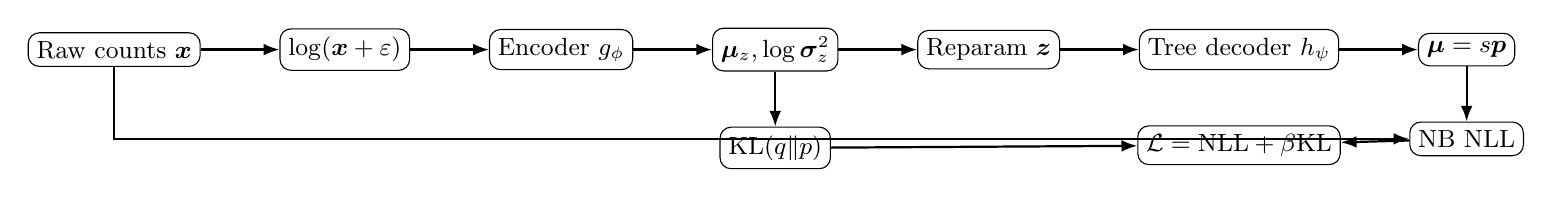
\begin{tikzpicture}[
  node distance=7mm and 10mm,
  box/.style={draw,rounded corners,align=center,inner sep=3pt,font=\small},
  arr/.style={-{Latex[length=2mm]},thick}
]
\node[box] (x) {Raw counts $\bm{x}$};
\node[box, right=of x] (logx) {$\log(\bm{x}+\varepsilon)$};
\node[box, right=of logx] (enc) {Encoder $g_\phi$};
\node[box, right=of enc] (q) {$\bm{\mu}_z,\log\bm{\sigma}^2_z$};
\node[box, right=of q] (z) {Reparam\ $\bm{z}$};
\node[box, right=of z] (dec) {Tree decoder\ $h_\psi$};
\node[box, right=of dec] (mu) {$\bm{\mu}=s\bm{p}$};
\node[box, below=of mu] (nb) {NB NLL};
\node[box, below=of q] (kl) {KL$(q\|p)$};
\node[box, below=of dec] (loss) {$\mathcal{L}=\text{NLL}+\beta\text{KL}$};

\draw[arr] (x) -- (logx);
\draw[arr] (logx) -- (enc);
\draw[arr] (enc) -- (q);
\draw[arr] (q) -- (z);
\draw[arr] (z) -- (dec);
\draw[arr] (dec) -- (mu);
\draw[arr] (mu) -- (nb);
\draw[arr] (x) |- (nb);
\draw[arr] (q) -- (kl);
\draw[arr] (nb) -- (loss);
\draw[arr] (kl) -- (loss);
\end{tikzpicture}
\end{center}

\subsection*{Tree factorization example}
\begin{center}
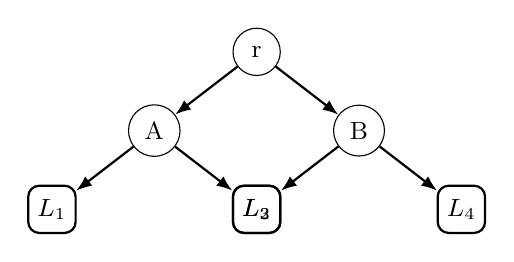
\begin{tikzpicture}[
  level distance=10mm,
  sibling distance=26mm,
  every node/.style={draw,circle,minimum size=6mm,font=\small},
  edge from parent/.style={draw,-{Latex[length=2mm]},thick}
]
\node (r) {r}
  child {node (a) {A}
    child {node[draw,rectangle,rounded corners] (l1) {$L_1$}}
    child {node[draw,rectangle,rounded corners] (l2) {$L_2$}}
  }
  child {node (b) {B}
    child {node[draw,rectangle,rounded corners] (l3) {$L_3$}}
    child {node[draw,rectangle,rounded corners] (l4) {$L_4$}}
  };
\end{tikzpicture}
\end{center}

For this tree,
\[
p_{L_1}=\pi_{r\to A}\pi_{A\to L_1},\quad
p_{L_2}=\pi_{r\to A}\pi_{A\to L_2},\quad
p_{L_3}=\pi_{r\to B}\pi_{B\to L_3},\quad
p_{L_4}=\pi_{r\to B}\pi_{B\to L_4}.
\]
So
\[
p_A=p_{L_1}+p_{L_2}=\pi_{r\to A},
\qquad
p_B=p_{L_3}+p_{L_4}=\pi_{r\to B}.
\]

\section{Summary}
TreeNB-VAE combines:
\begin{itemize}
  \item a Gaussian latent-variable encoder,
  \item a tree-factorized softmax decoder that guarantees exact hierarchical consistency,
  \item NB reconstruction with learned feature-wise dispersion,
  \item and a warm-started $\beta$-ELBO objective.
\end{itemize}

\end{document}
